
%% ==========================================================

The following chapter acts as a detailed introduction of the necessary background from literature.
First, different measurements that are utilized are introduced, 
both of which are generally used in e-commerce to measure success.
In addition to the measurements, the section introduces the testing platform utilized to collect the measurements
and to analyze the test results.

Second, the chapter introduces a search engine first at a more general level before introducing
Elasticsearch, the search engine utilized in this thesis, in more detail.
Lastly, the chapter introduces the ranking algorithms that served as a basis for the ones tested.
In addition to the ranking functions, the chapter introduces what the relevance of the search results means
as the purpose is to try to increase the conversion rate by offering more relevant search results to users.



%% ==========================================================
\section{Measurements in e-commerce}
\label{sec:measurements}

The most popular metric to measure the success of an e-commerce platform 
is a metric called conversion rate,
which provides a percentage of conversions compared to the total visitor count.
Despite measuring the performance of a website accurately, 
a drawback of conversion rate is that a great deal of data is necessary for it to be an accurate measurement 
\cite{conversionRateWhat}.
In addition, the overall conversion rate measures small changes poorly, 
since it measures the performance of the whole website, so
additional measurements are necessary to measure more specific changes.


For instance, to measure the performance of a specific element on a website, 
the usage of the conversion rate might be redundant. 
Moreover, the specific element might not have a noticeable effect on it, 
thus making the conversion rate inaccurate measurement for that situation.
For specific situations, there exists a metric called click-through rate (CTR), 
which can measure the performance a small change efficiently \cite{ctrWhat}.


The following sections provide an overview of the different measurements used in e-commerce relevant to this thesis.
First, Section \ref{ss:conversion} talks about the conversion rate in e-commerce, and second, 
Section \ref{ss:ctr} describes a metric called click-through rate.
Lastly, Section \ref{ss:abtest} provides an overview of the test platform that was used
when collecting the results of the implementations.


\subsection{Conversion rate}
\label{ss:conversion}
The overall conversion rate measures the proportion of orders to the website visitors \cite{conversionRate}.
For example, if a total of one hundred customers visit a website and two of them place orders, 
the conversion rate can be calculated with a formula
\[conversions\ /\ total\ visitors\ *\ 100\% = conversion\ rate \]
resulting in a conversion rate of 2\%.

Although the conversion rate is not commonly the most accurate metric to be measured, 
it generally is the most significant for an e-commerce organization.
The preceding example was with 100 visitors, which is a far too low number to measure conversion rate accurately \cite{conversionRateWhat}.
Furthermore, in the example, one more converting customer would increase the conversion rate by 50\%,
making the measurement highly inaccurate.


It is important to note that there are other types of conversion rates in e-commerce \cite{conversionRate}.
The above conversion rate calculates the overall conversion rate of an e-commerce platform.
In addition to placing an order, the conversions can be, for instance, form submissions, signing up for a subscription 
or events that product is added to cart \cite{conversionRateWhat}.
Depending on the situation, other types of conversion measurements might be necessary 
to capture effects that might not be shown by the overall conversion rate.
Furthermore, the same formula applies to the different types of conversion rates.


In this thesis, the measured conversion rate was the overall conversion rate of the e-commerce platform and 
the conversion rate of the proportion of customers who interacted with the search application.
Furthermore, the conversion rates were used as a metric to measure the performance of the search applications
compared to the baseline.


\subsection{Click-through rate}
\label{ss:ctr}

Click-through rate (CTR) is a measurement used mostly to measure the performance of a specific element on a website, 
for example, an advertisement \cite{ctrWhat}. 
CTR is calculated similarly to the conversion rate,
by dividing the conversions, which are the clicks on the element,
by impressions, which means the number of visitors, who have seen the element \cite{ctrWhat}.


While CTR measures the clicks on a single element accurately, the usage differs based on the situation.
Generally, high CTR means that the element is highly relevant. 
However, for instance, in an advertisement, ambiguous keywords might receive high CTR while not necessarily being relevant.
\cite{ctrWhat}

As mentioned above, the CTR can measure more specific changes in the element. 
Therefore, it was utilized to measure the performance of the search result list with different implementations.
Furthermore, to be more precise, to collect the number of clicks on the search results and the position, which product
was clicked on.
Since in each implementation, the product list is different, the CTR was able to capture the 
difference between implementations well and provide insight to the results.

\subsection{Measurements with production A/B testing}
\label{ss:abtest}

The measurements were an essential part of determining the performance of the introduced methods.
Furthermore, the measurements were collected by utilizing the Google Optimize platform to conclude A/B tests
to calculate the measurements during the tests from the collected data.
An A/B test is a randomized test where the test platform splits the website, or part of it, into two or more variants, 
and the platform redirects the traffic for the website into the different variants at random \cite{optimizeAbout}. 
Therefore, when testing the different implementations, the user interface of the search that the customer sees does not change. 
Only the search results presented to the customer differ.


Google Optimize is a test environment, but in addition to operating the tests, 
it provides a tool to see a rough estimate of the results of the tests, 
based on the goals defined for the test, without extensive analysis \cite{optimizeAbout}. 
The tool can give a quick estimate of the results,
which is useful in determining if the implementation was performing as expected. 
Furthermore, the goals of the tests utilized 
in this thesis are introduced later in Section \ref{sec:methodTests}.


In order to reliably infer if the concluded tests have increased the conversion rate, 
a detailed analysis of the results of the tests was necessary. 
Therefore, Google Analytics was utilized for this since it 
provides a detailed report about the test variants based on the metadata collected on the website
\cite{analyticsAbout}.
The organization already collects data about the performance of products and product lists, 
so utilizing the existing platform was a logical choice.


Generally, the metadata includes the click data when a customer browses the website, the purchase data, 
and the data, which products are shown on different pages to different customers.
The collected metadata can be utilized in both the configuration and the analysis of the tests 
by setting up custom goals for tests. 
Therefore, the completion percentage of the custom goal during a test can be analyzed.
The primary goals for e-commerce, for example, revenue and conversion, 
can be tracked with the completion of the custom goals.
\cite{analyticsAbout}
 

The above sections introduced the metrics used in this thesis and how the measurements are
collected.
Firstly, the conversion rate served as the primary measurement used in this thesis 
since it is generally the most utilized measurement in e-commerce.
Secondly, the click-through rate was introduced, which was utilized to measure more
specific changes.
In this case, the performance of the search result list.
Lastly, A/B tests were introduced and how they work and use the measurements to determine
the best result from the test variants.
The following sections move on to introduced search engines first on a more general level before
introducing Elasticsearch, the search engine platform used, in more detail.


%% ==========================================================
\section{Utilization of a search engine}

As a general term, a search engine means an application that performs a query from a user and 
presents the user with the results for the specified query. 
Furthermore, the era of modern search engines can be thought to have started when
\citeauthor{googleInit} \cite{googleInit} created Google,
now the largest search engine. 
Furthermore, Google has been a large part of making search engines part of our everyday life.
To further understand how a search engine is utilized in this thesis, this section
provides an overview in necessary detail.
In addition, this thesis uses Elasticsearch as the search engine; it shares a considerable amount
of similarities to the early search engine of Google introduced by 
\citeauthor{googleInit} \cite{googleInit}.
Elasticsearch is introduced in detail in Section \ref{sec:elasticsearch}, but the general
background of the search engines applies to it.


\subsection{Overview}

Generally, search engines must be able to search from extensive datasets efficiently.
A design goal of \citeauthor{googleInit} \cite{googleInit} in \citeyear{googleInit}
was to build a large-scale search engine 
that would be able to index hundreds of gigabytes of data, in addition to
performing hundreds of millions of queries per day.
The above numbers have grown exponentially in the last two decades, and a present-day
search engine might need to perform the same amount of queries every hour.

Searching from persistent storage or disk was not feasible, and a more efficient 
solution was necessary \cite{googleInit}. 
Thus, the design goals of \citeauthor{googleInit} \cite{googleInit} included the creation of 
a distributed indexing system, 
which they could efficiently store the documents. 
In addition, the indexing system needed to be able to process hundreds of gigabytes of data efficiently 
due to the queries from the users came in with a rate of hundreds to thousands in 
a second \cite{googleInit}. 
Furthermore, the preceding design goal set by \citeauthor{googleInit} \cite{googleInit}
over two decades ago,
describes an outline for many of the modern search engines, 
including Elasticsearch \cite{relevantSearch}.

A search engine is a complex application to do simple string matching efficiently
on a large-scale.
However, to perform in a simple task efficiently, a search engine requires a great deal of 
engineering work.
In some cases, a simple spelling mistake can result in an empty set of documents, thus creating 
frustration towards the search engine.
\cite{relevantSearch}

To simplify the complex application,
\citeauthor{ganSuel} \cite{ganSuel} broke down a web search engine 
to four different steps:
\begin{enumerate}
    \item Collecting the data from a source.
    \item Preprocessing the data to a specified format.
    \item Indexing the documents and creating an inverted index to the search engine.
    \item Processing queries and searching from the index.
\end{enumerate}
Despite describing a web search engine, the preceding steps can be applied to various 
search applications. 
First, during the data collection, the search application in this thesis 
collects the data from persistent storage, which includes multiple databases and database tables.
Second, since the data includes numerous unnecessary fields 
and only a selection of them is necessary, the collected data must be preprocessed.
Third, the previous step yields a document with a specified schema from the data, 
that is indexed with Elasticsearch Index APIs.
Indexing both stores the document and creates an inverted index from the document to the search engine.
Lastly, the queries are processed and sent to the search engine. 
Furthermore, the search engine performs a search against the inverted index and yields the results for the query.


While the four steps describe a search engine in more detail, 
\citeauthor{relevantSearch} \cite{relevantSearch} stated that 
a search engine consists of two major parts, the index time and the search time. 
Moreover, the first three steps are considered as the index time, which is described in Section \ref{ss:invertedIndex},
and the fourth step is the search time, described in Section \ref{ss:searchTime}.

\subsection{Creating the inverted index}
\label{ss:invertedIndex}

The inverted index is a central data structure of a search engine enabling 
matching query terms to the documents swiftly.
In worst cases, the fields in documents can contain an extensive amount of text, so 
finding a match from the documents can be costly.
The inverted index is created to solve the problem of going through all the documents 
every time a query must be performed. \cite{relevantSearch}


The inverted index consists of two crucial parts a terms dictionary and a postings list \cite{relevantSearch}.
\citeauthor{relevantSearch} \cite{relevantSearch} introduced the following listings
describing how the inverted index is created in Elasticsearch.
The listing \ref{lst:docs} includes the example documents, which are indexed to a search engine.
\begin{lstlisting}[
caption={Example text documents with identifiers \cite{relevantSearch}.},
captionpos=b,
label={lst:docs},
frame=single]
    0. One shoe, two shoe, the red shoe, the blue shoe.
    1. The blue dress shoe is the best shoe.
    2. The best dress is the one red dress.
\end{lstlisting}
During indexing, a term dictionary (\ref{lst:terms}) is created by collecting all individual
terms called tokens from the documents. 
Furthermore, each of the terms has an identifier, which maps the term to the posting list (\ref{lst:postings}).
\begin{lstlisting}[
caption={Term dictionary is generated from terms in the documents \cite{relevantSearch}.},
captionpos=b,
label={lst:terms},
frame=single,
mathescape=true,
literate={=>}{$\rightarrow$}{1}
]
    best  => 0      red   => 5
    blue  => 1      shoe  => 6
    dress => 2      the   => 7
    is    => 3      two   => 8
    one   => 4
\end{lstlisting}
\begin{lstlisting}[
caption={Postings list is a mapping between the term dictionary and documents
\cite{relevantSearch}.},
captionpos=b,
label={lst:postings},
frame=single,
mathescape=true,
literate={=>}{$\rightarrow$}{1}
]
    0 => [1,2]      5 => [0,2]
    1 => [0,1]      6 => [0,1]
    2 => [1,2]      7 => [0,1,2]
    3 => [1,2]      8 => [0]
    4 => [0,2]
\end{lstlisting}

In addition, the inverted index in Elasticsearch contains additional metadata necessary during the query evaluation
\cite{relevantSearch}. 
\citeauthor{relevantSearch} \cite{relevantSearch} provided a full list of the metadata, and
the following list introduces a selection of the metadata from the list necessary for this thesis.
\begin{itemize}
    \item \emph{Document frequency} is a count of documents that contain the term, thus 
    establishing a notion of the importance of the term. 
    Generally, the higher the document frequency indicates that the term provides little value when 
    determining the relevance of the document to a query.
    For instance, the term \enquote{the} has a high document frequency providing little value 
    for the relevance calculation.
    \item \emph{Term frequency} determines how many times the term occurs in a document
    providing a notion of how well a query matches the document.
    In a nutshell, document 0 contains the term \enquote{shoe} four times and document 1 two times,
    making the document 0 twice as important match for the query term.
    \item \emph{Term positions} provide the position where the term occurs in a document. 
    It makes finding documents with phrase matching possible.
    \item \emph{Term offsets} keep track of the start and end character offsets. 
    For example, Google search provides highlights of the matches in the search result listing,
    which keeping track of the term offsets enables.
    The highlights provide feedback to the user on why the result matched the query.
    \item \emph{Stored fields} contain the necessary fields used during searching. 
    The fields in the inverted index are scrambled versions of the original document, and all fields 
    presented back to the user must be separately saved to the stored fields.
    Therefore, the fields might require a great deal of disk space depending on the size of the fields.
    \item \emph{Doc values} usually contain auxiliary values relevant to scoring the search results.
    For instance, the values used in sorting or boosting the results are stored in the doc values.
\end{itemize}

The above section provided an overview of the inverted index, the primary data structure of the search engine.
In addition, the data saved to the inverted index was introduced, as it is referenced in later chapters.
The following section continues to describe what index time means and how the inverted index is 
created in index time.

\subsection{Index time}
\label{ss:indexTime}

The index time can be viewed as an extracting, transforming, and loading information (ETL) pipeline \cite{relevantSearch}.
Furthermore, ETL pipelines are referred to when moving data from storage to another while processing it in between \cite{relevantSearch}.
In this thesis, the ETL pipeline steps for moving the data from persistent storage to the search engine are shown in Figure \ref{fig:etlPipe}.

The steps of the pipeline are extraction, which collects the product data from the persistent storage.
After the collection, the data is enriched with the additional data necessary to be searched.
Furthermore, Figure \ref{fig:etlPipe} shows the description of the product and impressions, which is the number of times the product has been viewed, both utilized in searching. 
The former, when matching the search query to a product, the latter, by the ranking algorithm in the relevance calculation.


\begin{figure}
    \centering
    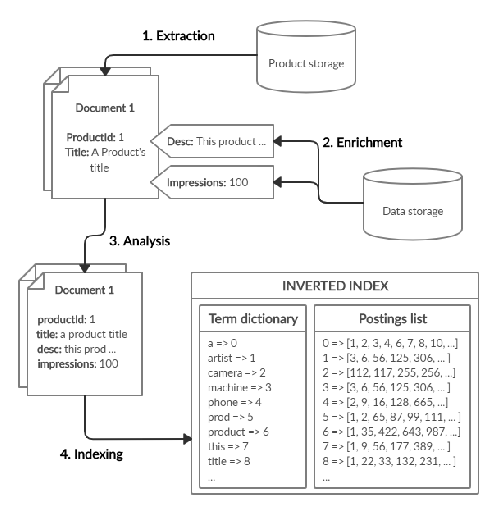
\includegraphics[scale=1.5]{img/etl-pipeline.eps}
    \caption{Index time described as an ETL pipeline \cite{relevantSearch}.}
    \label{fig:etlPipe}
\end{figure}

The third step is analysis, which in Elasticsearch happens during the indexing.
Before the metadata described in Section \ref{ss:invertedIndex} is collected from the document, 
a set of analyzers are utilized to create better terms \cite{elasticIntro}.
For instance, Figure \ref{fig:etlPipe} shows that all text from the document is lowercased, and 
the possessive ending from the title of Document 1 is removed \cite{relevantSearch}.
Elasticsearch does this by default to normalize the search terms to make the documents easier to find \cite{elasticIntro}.
In an ideal case, after the analysis step, a term with plural should match the term without one, thus, 
making both documents match a query with the term.
This thesis utilizes a set of analyzers to generate more generic search terms for specific fields.
Furthermore, the analyzers used are introduced in Section \ref{ss:textAnalysisTools}.


The last step of the ETL pipeline is to index the analyzed documents.
Furthermore, indexing is the process that saves the data to the inverted index and the storage of the search engine \cite{relevantSearch}.
Generally, the focus during indexing is on the computation performance and resource management
since the more the fields from the documents are analyzed, the slower the indexing becomes 
requiring more storage computation power and storage \cite{relevantSearch}.
In Elasticsearch, the analysis and the indexing happen automatically when 
a document or a set of documents is posted to the Index API \cite{elasticIntro}.

Searching from the field becomes available only when the field is indexed.
Consequently, making the decision between which fields to index, which to store, or which fields both index and store.
Storing the fields refers to saving original content to the metadata data structure introduced in Section \ref{ss:invertedIndex}.
\cite{relevantSearch}


As mentioned above, the utilization of a search engine can be divided into two parts, index time and search time.
The above section introduces what index time is and how the inverted index is created.
Furthermore, the following section continues to introduce what search time is and how 
the documents are searched from the index.


\subsection{Searching from the index}
\label{ss:searchTime}
A search engine is not an intelligent machine; instead, it is merely a text-matching tool \cite{relevantSearch}. 
When a query is submitted to the search engine, it 
matches the individual terms from the query to the tokens in the inverted index, 
which consequently map to the documents in the index \cite{relevantSearch}. 
Inverted index functions like the index from the end of books, 
where the reader can look for a specific topic and find the relevant page number \cite{relevantSearch}.
Searching for a specific subject from a book by going through page by page is not efficient.
Instead, the relevant pages can generally be found from the index much faster.
Furthermore, the same applies to the search engines;
the abundance of data generally makes searching the documents one by one unfeasible.


After a term matches a document, a content score for the match is calculated based on the metadata values in the index
\cite{relevantSearch}.
The content score determines how good of a match the document is to the query.
In addition to the content score, additional business scores can be calculated for the document to provide 
additional measurements of relevance.
Furthermore, the search engine sorts the resulting list in an order specified in the query, and generally, 
by default, the score determines the order of the resulting list. 
Thus, yielding in a list sorted by the relevance of the search result.


While the previous section provided an overview of the basic functionalities of a search engine,
the following section discusses how Elasticsearch works and how the functionalities are utilized in this thesis.
First, the section provides an overview of Elasticsearch, before moving on the various text analysis 
utilized when implementing the new search functionalities to the current search application.
Lastly, the section describes how the results are searched and scored in Elasticsearch before they 
are returned to the user.

%% ==========================================================

\section{Elasticsearch as a search engine}
\label{sec:elasticsearch}
This section discusses how Elasticsearch works and how the functionalities are utilized in this thesis.
First, the section provides an overview of Elasticsearch, before moving on the various text analysis 
utilized when implementing the new search functionalities to the current search application.
Lastly, the section describes how the results are searched and scored in Elasticsearch before they 
are returned to the user.


Elasticsearch provides real-time search and analytics for all types of data.
The data is stored and indexed in a way that fast searches are supported.
In addition, Elasticsearch provides a possibility to go far beyond simple information retrieval and supports
different aggregations to fetch data efficiently. 
The distributed nature of Elasticsearch provides additional resiliency when the volume of the data 
grows. 
\cite{elasticIntro}


The power of Elasticsearch comes from the optimally indexed data structures; for instance, text fields are by default
indexed as inverted indices with the tokens collected from the fields of the documents.
Elasticsearch enables saving the data to different kinds of data structures depending on the use cases.
For example, an analyzer can be applied to process data from a specific field,
which creates an own data structure for the field with the data collected by the analyzer.
\cite{elasticIntro}


The following part of this thesis describes, in greater detail,
the text analysis tools provided by Elasticsearch utilized in this thesis.
An understanding of these tools is necessary because they are used in 
the methods introduced in Section \ref{ch:methods}.



%% ==========================================================
\subsection{Text analysis}
\label{ss:textAnalysisTools}

Text analysis in Elasticsearch means transforming text to tokens, which are stored in the inverted index.
Choosing how the text is transformed determines the performance of the search application.
During the analysis, the search engine converts the data from the documents into tokens using analyzers
and stores the tokens in the internal data structures of the search engine.
Besides utilizing analyzers to the documents while indexing, 
the queries can be analyzed with the same analyzers.
\cite{relevantSearch}

As previously stated, search engines are merely trying to find exact matches the query from the
inverted index. 
Without good tokens in the inverted index,
the document can be challenging to find with a query that might not exactly match the document.
To make the documents more findable, Elasticsearch provides various analyzers by default and provides
the capability to create custom analyzers from different tokenizers and token filters 
\cite{relevantSearch}.


In some languages, such as Finnish, there are various inflected forms for a word, which can make
matching the document to the query more difficult.
The analyzers can help by stemming the search term, which means reducing the term into its root form \cite{relevantSearch}.
For instance, stemming the terms \emph{foxes} and \emph{jumped} to root forms \emph{fox} and \emph{jump}.


Generally, in e-commerce, the users might not use the most effective search terms to describe
what they are searching for, instead of using technical terms, they use familiar terms.
By reducing all words from documents and search queries into root forms, the products better match
the search terms used by the customers \cite{relevantSearch}.
Furthermore, interacting with a search application that does not understand what is being asked from it
can make users frustrated and might negatively affect their experience on the website \cite{relevantSearch}.

The following section focuses on 
how tokens are generated with analyzers provided by Elasticsearch relevant to this thesis.
Additionally, a selection of the tokenizers and token filters is introduced since a custom
analyzer had to be created to provide the functionality necessary for this thesis.

%% ==========================================================
\subsubsection{Extracting features from text}
\label{ss:extrackingFeatures}

While token generation is a crucial part of a search application, it is essential to note that the tokens should not 
merely be the words from the text.
Since the tokens are the parts that the search engine is going through when a query is received, the tokens
should try to capture the meaning of the text instead of the text itself to make query matching more robust.
Furthermore, tokens should try to anticipate the expectations of the user, which can lead to 
highly relevant and targeted results.
\cite{relevantSearch}

In feature modeling, the purpose is to take into consideration the intent of the user, 
in addition to the ideas conveyed in the indexed documents.
Additionally, feature modeling ensures that the generated tokens represent the descriptive and meaningful
features of the queries making understanding the information in the documents as well as the intent of the users.
For instance, useful features take into account the pluralization and the parts of speech in addition to the specific language
used in the domain context to make the query and the tokens match.
When the features capture both the meaning of the document and the query well, 
the matches become increasingly relevant.
The feature modeling is done in both the index and the search time, so the meaning of the term is captured consistently.
\cite{relevantSearch}

The feature modeling, among many other optimization tasks, is a constant battle between 
precision and recall \cite{relevantSearch}.
In a search application context, precision describes the percentage of documents in the results 
that are relevant to a query, and recall means the percentage of the relevant documents in the results
\cite{relevantSearch}.
Precision is calculated with the following formula
\[ precision = doc_{relevant} / (doc_{relevant} + doc_{irrelevant}) \]
where the $doc_{relevant}$ and $doc_{irrelevant}$ are
the numbers of relevant and irrelevant documents in the matches,
respectively recall is calculated with the formula
\[ recall = doc_{relevant} / (doc_{relevant} + doc_{relevant_{no match}}) \]
where the $doc_{relevant}$ describes the number of relevant documents in results, 
and $doc_{relevant_{no match}}$ is the total number of relevant documents that do not match
the query.
Generally, higher precision means lower recall and vice versa, which implies there is an optimal threshold 
that could be achieved with optimization.
In an ideal case, both precision and recall would be 100\%, but that is nearly impossible \cite{relevantSearch}.


In this thesis, the trade-off between precision and recall appeared in one of the empirical tests 
chosen to measure the relevance in the development process.
In Finnish, all terms
\emph{pyykinpesukone}, \emph{kuivaava pesukone} and \emph{astianpesukone} 
are separate product categories, and the query ``pesukone`` was quite common.
However, most certainly, the major part of Finnish speakers would tell that ``pesukone`` does not mean 
\emph{astianpesukone}, and most likely, the best match would be \emph{pyykinpesukone}, or 
at least it should be included near the very top of the results.
By exactly matching ``pesukone`` to a term in the inverted index increases precision as only \emph{kuivaava pesukone} category 
is included, but decreasing recall as the \emph{pyykinpesukone} category is left out from the product lists.
Vice versa, if ``pesukone`` matches all words that contain it, the precision is decreased, and recall increased as all
three categories are included.

Teaching a search engine to know that a query 
should not only match the exact word found from the inverted index 
but to one word which does not start with the query itself can swiftly become an optimization problem.
Generally, similar problems are not easily solvable in practice but somewhat
tedious and time-consuming to solve and might need additional feature extraction.


% In summary, this section introduced the importance of feature modeling in analysis and 
% how it can be found in practice by giving an example of a problem found during development.

% Furthermore, the following sections introduce analyzers, which are the tools responsible
% for collecting the tokens from the documents.


%% ==========================================================
\subsubsection{Analyzers}

This section introduced different analyzers, which are the tools responsible
for collecting the tokens from the documents.
In Elasticsearch, an analyzer is used in the text analysis step to extract tokens from the documents \cite{elasticIntro}.
The usage of the analyzer is configurable, and multiple analyzers can be used for each field \cite{relevantSearch}.
Even though there can be multiple analyzers defined for a field, only one can be utilized at a time
because each of the analyzers creates a new inverted index from the field \cite{relevantSearch}.


A drawback when creating analyzers is that configuring them requires the index re-creation, making changing the analyzers 
on an existing application complicated.
For instance, if a search application uses index A, then a new index B must be created, and 
all documents must be re-indexed,
after which the search application can be told to use the new index B.
Creating multiple indices can cause issues in some data-sensitive applications because of the index creation, 
and data replication is not instantaneous.


Analyzers allow normalization of tokens to create common representations to overcome the limitations of the byte-by-byte
matching ability of the inverted index \cite{relevantSearch}.
Furthermore, analysis enables expressing the essential features of the search application as tokens \cite{relevantSearch}.
The analyzers consist of tokenizers and token filters, and Elasticsearch provides a selection of 
built-in analyzers \cite{elasticIntro}.
A custom analyzer can be created and can be useful in specific situations in extracting the tokens from 
a field.
For instance, parts from an email address can be extracted to create tokens from it, 
which can make searching for the email more efficient \cite{relevantSearch}.


In Elasticsearch, a standard analyzer is used if none other is specified, and 
it is typically the first analyzer used in a search application \cite{elasticIntro, relevantSearch}.
The standard analyzer divides input text into tokens on word boundaries, defined
by the Unicode Text Segmentation (UTS) algorithm, and works well for most languages \cite{elasticIntro}.
Besides creating tokens from the input, the analyzer converts all the tokens to lowercase \cite{elasticIntro}.
Typically, the standard analyzer results have high precision, but low recall
since it does not capture features of the text well, and user query must match the document exactly
\cite{relevantSearch}.


The language analyzers work similarly to the standard analyzers. 
However, there are some minor differences between the languages 
provided by Elasticsearch by default.
For instance, the English analyzer will convert the following sentence:
\begin{lstlisting}[
caption={Input for the English analyzer \cite{elasticIntro}},
captionpos=b,
label={lst:analyzerInput},
frame=single]
    The QUICK brown foxes jumped over the lazy dog!
\end{lstlisting}
into distinct tokens, convert all text to lowercase, remove the stop words, and
additionally stemming the words (see Section \ref{ss:textAnalysisTools}).
The output of the analyzer is the following list of terms that are added to the inverted index:
\cite{elasticIntro}
\begin{lstlisting}[
caption={Output of the English analyzer \cite{elasticIntro}},
captionpos=b,
label={lst:analyzerOutput},
frame=single]
    [ quick, brown, fox, jump, over, lazi, dog ]
\end{lstlisting}


As shown in the example above, the language analyzers try to capture the meaning of the words and 
carry the meaning to the inverted index \cite{relevantSearch}.
A search engine is merely a token-matching system that does not know 
about the meaning of the tokens \cite{relevantSearch}.
The purpose of analyzers is to capture the meaning and the intent of the user to make better tokens 
\cite{relevantSearch}.
The built-in analyzers may not be enough for specific application domains
or may perform poorly on some languages.
In Elasticsearch, the tokenizers and token filters, introduced in the following sections, 
facilitate the building of customer analyzers to target specific issues with the built-in analyzers.


%% ==========================================================
\subsubsection{Tokenizers}


Tokenizers create the tokens from input words.
A tokenizer receives a stream of characters as an input and dismantles them to tokens and outputs a stream
of tokens \cite{elasticIntro}.
In addition, tokenizers are responsible for collecting the position of each term, and the start 
and the end character offsets of the original word that the term represents 
to be saved to the inverted index (Section \ref{ss:invertedIndex}) \cite{elasticIntro}.
The collected positions are used in a phrase or word proximity queries, and 
the start and end character offsets are utilized in highlighting the matches in the
search results \cite{elasticIntro}.
Two different tokenizers, a standard tokenizer and 
an edge-N-gram tokenizer, were utilized in this thesis.


As explained earlier, the standard and language analyzers divide the words into tokens,
both utilize standard tokenizer in doing that. 
Rather than creating the tokens, the analyzers utilize tokenizers and token filters in token creation.
The standard tokenizer uses the UTS algorithm to divide the text,
and it also removes punctuation symbols from the input.
The standard tokenizer works well in most languages, and it is used as the default in Elasticsearch.
\cite{elasticIntro}


The is edge-N-gram tokenizer first divides the text into words when encountering
specified characters, for instance, whitespace or punctuation. 
Then, the tokenizer returns an N-gram of the single word anchored to the start of the word.
$N$ means the maximum amount of characters in the resulting output of the tokenizer.
For instance, Listing \ref{lst:edgeNGramInput} shows the input to the edge-N-gram tokenizer, and
Listing \ref{lst:edgeNGramOutput} shows the output with $N = 5$, where the words are divided into tokens 
with a minimum of two characters and a maximum of five characters.
\begin{lstlisting}[
caption={Input to the edge-N-gram tokenizer \cite{elasticIntro}},
captionpos=b,
label={lst:edgeNGramInput},
frame=single]
    Quick Foxes.
\end{lstlisting}
\begin{lstlisting}[
caption={Output from the edge-N-gram tokenizer \cite{elasticIntro}},
captionpos=b,
label={lst:edgeNGramOutput},
frame=single]
    [ Qu, Qui, Quic, Quick, Fo, Fox, Foxe, Foxes ]
\end{lstlisting}
Elasticsearch allows the minimum and maximum characters N to be configured along with the characters 
that should be included in the generated tokens.
\cite{elasticIntro}


The built-in language analyzers perform poorly on some languages, which became
a problem during the development of the new search functionalities.
The Finnish language analyzer had a hard time capturing some of the plural forms in the Finnish language.
For instance, capturing the features from the words \emph{langaton} and \emph{langattomat} was difficult,
because of the addition `t` character added in the plural form of the word wireless.


In this thesis, an edge-N-gram tokenizer was utilized in generating the tokens from text to solve the problem described above.
The aim was to mimic the behavior of the language analyzer and try to capture the meaning of the words
by capturing the start characters.
While the usage of edge-N-gram tokenizer increased the recall of the search results, 
it quickly decreased the precision since if the minimum length for a token were defined too low,
the results would include almost all searchable products.
Before the generated tokens are added to the inverted index, a set of token filters
should be applied.


%% ==========================================================
\subsubsection{Token filters}


Token filters are an essential part of the analysis process since the tokenizers are not enough to generate
consistent tokens to the inverted index.
Since tokenizers do not modify the words, only divide them, the purpose of token filters is
to create consistent tokens by modifying the stream of tokens output by a tokenizer.
Furthermore, Elasticsearch provides various built-in token filters \cite{elasticIntro}. 
Token filters relevant to this thesis are introduced below.


\begin{itemize}
    \item \textbf{Lowercase token filter} modifies the stream of tokens and converts the characters to lowercase,
    making the tokens consistent and enabling case insensitive queries.
    A lowercase filter is in the core of every built-in analyzer Elasticsearch offers.
    
    \item \textbf{ASCII folding token filter} converts the alphabetic, numeric, and symbolic Unicode characters
    to ASCII characters, if one exists. 
    Utilizing it allowed the queries to match the words regardless if Scandinavian characters such as 'ä' instead of 'a' was used.
    Generally, all search engines utilize a similar functionality to match documents regardless
    of the special characters.
    
    \item \textbf{Edge-N-gram token filter} implements the same functionality as the edge-N-gram tokenizer.
    The need for using the token filter instead of tokenizer is if additional token filters are needed before splitting the tokens
    into N-grams.
    For instance, the edge-N-gram from the end of the word must utilize the token filter, since the 
    words must be reversed with a filter before generating the N-gram.
    
    \item \textbf{Conditional token filter} uses a condition and a list of subfilters and applies the 
    subfilters to the token only if the token matches the condition returning otherwise the original token.
    For this thesis, a search time edge-N-gram filter was created, which used a condition to determine 
    the length of the search term.
    If the search term was longer than the average length search term, which was 6, 
    a subfilter applied an edge-N-gram token filter to the term.
    
    \item \textbf{Stemmer token filter} is used in the language analyzers to try to capture the
    meaning of the word by trying to collapse multiple forms of the same words into one.
    Furthermore, the token filter is available in multiple languages.
    
    \item \textbf{Stop token filter} uses a predefined set of stop words to filter out from the tokens.
    For instance, the words ``and`` and ``the`` do not bring meaning to the search since they are too common.
    So, a token filter removes those altogether from the inverted index to make it more compact.
    
    \item \textbf{Unique token filter} is used to remove the duplicate tokens from the token stream. 
    So, if a text has multiple duplicate terms, which bring no value, then this filter could be applied.
    Since the usage of this filter may affect the scoring of the documents, 
    it should be used only to bring additional tokens to the index from the fields, 
    where duplicates are irrelevant.
    
\end{itemize}


% This section has provided a detailed overview of the text analysis tools relevant to the thesis.
% The tools introduced here were used to build a custom analyzer that was designed to capture 
% the features from the words similar to the language analyzer, but additionally to generate smaller tokens
% to make the matching easier.
% In addition to the usage of the text analysis tools in search time,
% the section that follows introduces the necessary search functionalities of Elasticsearch.


%% ==========================================================
\subsection{Searching with Elasticsearch}
\label{ss:searchElasticsearch}


In addition to the text analysis tools, Elasticsearch supports complex queries and provides
analyzing capabilities to the queries \cite{elasticIntro}.
This section introduces briefly how the queries can be used to collect metadata about the results 
and what is the difference between the filter and the query context, 
before continuing to more specific parts of the search time.


The metadata about the results that match the query is collected with aggregations, 
also known as facets \cite{elasticIntro}.
A typical use case for aggregations is the filters in lists on websites.
Aggregations allow the query to collect data about the matching documents 
while searching the results from the inverted index without returning all the results to 
the end-user \cite{relevantSearch}.
For instance, the number of products in individual categories can be collected and constructed to 
a search filter shown on the search result page.
\citeauthor{relevantSearch} \cite{relevantSearch} recommend that every website should have
a selection of filters in product lists.
However, the aggregations are out of the scope of this thesis, since the current search application already
utilizes them.
The filters also provide useful feedback to the user about
the results of the submitted query \cite{relevantSearch}.


While querying in Elasticsearch, there are two different contexts filter and query. 
The filter context tells whether the document matches a query
by returning a boolean value, which is used to filter out the documents from the results \cite{elasticIntro}.
The query context tells how well the document matches a query,
providing a relevance score about the match \cite{elasticIntro}.
The relevance score, also known as the content score, is used by scoring functions
to reflect the score for the content, and additional business scores can be added to it \cite{elasticIntro}.

Since the relevancy score is calculated based on the query context, it is to differentiate
the requirements a document must fulfill to the filter context.
Otherwise, it can affect the relevancy score of the document in an unexpected way.
For instance, the current search application has multiple rules that a product must match 
before it should be in the search results. 
Most of these rules define if a product is active.
If the rules are constructed into the query rather than as a filter, they
distort the actual relevance score of the documents, 
which in some cases can lead to unexpected scoring of the results.


% While this overview provided a brief introduction to how searching works in Elasticsearch,
% the following part provides additional detail on the necessary subjects.
% Firstly, the query syntax differs from the syntax, traditionally used in information retrieval. 
% Secondly, how the text analysis tools introduced in Section \ref{ss:textAnalysisTools}.
% Lastly, the different scoring functions built-in to Elasticsearch and how those were
% utilized in this thesis to create a custom ranking algorithm for the search application. 



%% ==========================================================
\subsubsection{Query syntax}

Searching in Elasticsearch is made through the Query API, which relies on Lucene \cite{elasticIntro}.
Lucene is a search engine software library developed by Apache.
Lucene supports various types of data collection techniques in addition to 
the basic information retrieval queries \cite{relevantSearch}.

The Lucene query syntax differs from the syntax, traditionally used in information retrieval.
For instance, the basic boolean query operators (AND/OR/NOT) are implemented as Lucene operators (MUST/SHOULD/NOT).
While the basic functionalities are like the basic boolean operators, 
the Lucene operators provide more flexibility than the basic methods.
Because the individual operators describe the operation for individual terms instead of the relationship between the terms,
the query with basic boolean operators is generally more complex than the same query with Lucene operators.
\cite{relevantSearch}

Listing \ref{lst:luceneOperations} shows a query with Lucene query syntax, where a matching document must contain a term \emph{cat},
should contain a term \emph{black}, and must not contain a term \emph{dog}.
The same query can also be implemented with the basic boolean operators.
Listing \ref{lst:basicOperations} shows that the query becomes more complex and is not as readable as with the Lucene operators.
\cite{relevantSearch}
\begin{lstlisting}[
caption={Example query with the Lucene operators \cite{relevantSearch}},
captionpos=b,
label={lst:luceneOperations},
frame=single]
    black +cat –dog
\end{lstlisting}
\begin{lstlisting}[
caption={Example query with the basic boolean operators \cite{relevantSearch}},
captionpos=b,
label={lst:basicOperations},
frame=single]
    (cat OR (black AND cat)) AND NOT dog
\end{lstlisting}


From a relevance standpoint, the MUST operator provides more relevant results to the query 
yielding in documents that match all parts of the query \cite{relevantSearch}.
However, the operator also returns no results if a document does not contain all terms present in the query \cite{relevantSearch}.
Since showing search pages with zero results to customers in an e-commerce application should be avoided \cite{zeroResults},
the SHOULD operator might be more applicable in some cases, because it provides resiliency against spelling mistakes.
Since the search application currently utilizes only MUST operators, a test with SHOULD operators was concluded
to confirm the presumption that the MUST provides more relevant search results in the current e-commerce search application.



%% ==========================================================
\subsubsection{Matching search terms to tokens}
\label{ss:matchingTokens}

When a query is submitted, the same analyzers that were applied when the index was created, 
are usually applied to the search terms to make the tokens consistent
\cite{relevantSearch}.
Analyzers used by default, both in index time and in search time, are standard analyzers for text fields,
but the analyzer that should be used for a specific field can be changed when constructing the query
\cite{elasticIntro}.
By default, if an analyzer is specified, the same analyzer is used both in index time and in query time.
However, a different search time analyzer can be defined when creating the index, making the search engine
use different analyzer for the search term as used while indexing the document \cite{relevantSearch}.


In this thesis, a different search time analyzer was necessary for the custom analyzer to restrict 
the generation of the N-grams in the search terms. 
Most of the problems of the language analyzer were caused by not capturing the features
from longer than average search term well.
The custom N-grams were only generated from longer terms in search time 
while allowing the generation of smaller tokens in index time.
When the N-grams were generated from shorter words, the recall of the search increased.
However, the precision of the search results decreased significantly as more irrelevant matches were included.


To enable the search-as-you-type feature or to search with incomplete search terms, a wildcard search is 
a useful tool \cite{relevantSearch}.
It provides the possibility to add a '*'-sign to the end or the start of the search term, which matches one or more
terms and enables the search with incomplete search terms or additionally can help to solve search problems like
the one introduced in Section \ref{ss:extrackingFeatures}.


However, the overuse of wildcards can introduce a relevance problem, where the recall increases, and 
the precision decreases, especially when wildcards are added to both ends of a shorter search term. 
The current solution adds a wildcard to the start and end of each term, which turned out to be necessary
due to the current limitations of the content like the example in Section \ref{ss:extrackingFeatures}.
To solve the problem of providing low precision, an implementation that boosts exact matches
by adding a score to them was created.
The query ranked more relevant content closer to the top of the search results, thus, increasing
the relevance of the top search results.


Another functionality, which enabled the searching with incomplete terms, 
is fuzzy search \cite{relevantSearch}.
Fuzzy search matches the tokens that are similar to the search term \cite{elasticIntro}. 
The similarity is determined by calculating the one-character 
changes necessary to match the search term to a token in the inverted index \cite{elasticIntro}.
A fuzzy search creates a set of all possible variations from the search term within a specified edit distance
and uses them to find matches from the inverted index \cite{elasticIntro}.
For instance, the variations include changing, removing, or inserting characters, or transposing two adjacent characters 
\cite{elasticIntro}.


While the fuzzy search is designed to fix the typing errors of the search terms, 
there are other ways to factor in the typing errors, 
such as the search term suggestion, which is included in this thesis instead of the fuzzy search.
During the implementation, the fuzzy search was investigated.
However, a similar problem with precision and recall arose as it did with the edge-N-gram. 
If the fuzziness was included in shorter search terms, 
too many irrelevant results were found, due to the static edit distance.
In addition, the fuzzy search cannot be used with the wildcard search \cite{elasticIntro},
which the current solution relied on heavily.
For these reasons, the fuzzy search was replaced with term suggestion, when no results were found.
The results showed that suggesting and automatically searching with a term was effective.
Therefore, the fuzzy search might be beneficial and should be investigated further and probably included and tested 
in the future.



%% ==========================================================
\subsubsection{Scoring documents}

This section introduces scoring functions that are provided by Elasticsearch and 
how the score for the documents is calculated.
As a base in the content score calculation in Elasticsearch is the following formula
\[ term\ frequency\ \times\ inverse\ document\ frequency \]
to calculate how well a term matches a document \cite{relevantSearch}.
A high score indicates that the word is important to a document.
Both frequencies are already collected during indexing, as introduced 
in Section \ref{ss:invertedIndex}.
Optionally, the base calculation can be changed, but in this thesis, it was not necessary.


\citeauthor{relevantSearch} \cite{relevantSearch} argue that relevant search results in the e-commerce
context must not only meet the needs of the user but also meet the needs of the business.
To achieve this, besides a content score, a business score must be added to the document
\cite{relevantSearch}.
To apply additional scores to the documents, Elasticsearch provides built-in scoring functions
to create compound queries \cite{elasticIntro}.
The compound queries wrap other queries inside them to either combine the resulting scores
or to switch from the query to the filter context \cite{elasticIntro}.


This thesis utilizes two types of compound queries that are boolean queries and function score queries.
The boolean queries are the default query type for combining multiple queries with the query clauses 
\emph{must}, \emph{should}, \emph{must\_not}, and \emph{filter} \cite{elasticIntro}.
The first three boolean queries map to the Lucene query syntax and last means to the filter context. 
For instance, each of the query clauses is used in the current rules about product activity, as mentioned
earlier.
In the boolean queries \emph{must} and \emph{should} clauses are executed in the query context, 
and \emph{must\_not} and \emph{filter} clauses are executed in the filter context \cite{elasticIntro}.


The function score queries are utilized in the ranking function implemented in this thesis.
It provides the ability to modify the content scores returned by the main query and
takes into account other configured functions when calculating new scores for the document \cite{elasticIntro}.
Figure \ref{fig:function_score} provides an example of a function score query that was tested 
during the development phase of this thesis.
The function score query wraps the main query inside, seen on line 15 of the figure, 
and adds results of several mathematical functions to the resulting content scores from the inner query.


\begin{figure}
    \centering
    \includegraphics[width=\textwidth]{img/function_score.png}
    \caption{Example of a functions score query tested in this thesis.}
    \label{fig:function_score}
\end{figure}


The function score query provides a possibility to define
how the scores from the individual functions are combined \cite{relevantSearch}.
Figure \ref{fig:function_score} shows the query has \emph{sum} as the \emph{score\_mode}, which calculates
the scores for the documents with the following formula \cite{relevantSearch}
\[ score_{total} = w_1 \times score_{views} + w_2 \times score_{orders} + w_3 \times score_{content} \]
The field value factor functions fetch a decimal value from the document and use it as the score
for the functions. A missing value from the document is replaced
with the value defined in the missing parameter \cite{elasticIntro}.


The above formula uses weights for each value when calculating the total score to enable dynamically 
changing the weight of the different functions \cite{relevantSearch}.
The weights from the formula can also be seen in Figure \ref{fig:function_score}.
The individual weights are defined inside each function (Figure \ref{fig:function_score}), and the last weight
in the figure is the content weight $w_3$ presented.
As was stated before, the ranking of the search results is an optimization problem, and finding
the optimal threshold can be automated to find the optimal solution by testing different weights.


Figure \ref{fig:query_string} shows an example query that was used during development.
This query utilizes a query string query provided by Elasticsearch.
The query string query allows the creation of complex queries that include wildcard characters,
searching across multiple fields, and the usage of different functionalities.


\begin{figure}
    \centering
    \includegraphics[]{img/query_string.png}
    \caption{Example query used in this thesis.}
    \label{fig:query_string}
\end{figure}


The example query defines a structured search across multiple fields as an array of field names.
The query uses boosts on the individual fields \emph{title} and \emph{manufacturerName}.
In Elasticsearch, the boost for a specific field is defined with a circumflex followed by the multiplier
that multiplies the base content score for the field \cite{relevantSearch}.
In addition to field boosts, the example query utilizes the previously introduced search time 
edge-N-gram analyzer to match the term to a category and the manufacturer of the product.


The search terms are shown in the query variable.
Both terms are surrounded by the wildcard characters to allow the terms to be matched with
characters missing from either end.
A query must enable \emph{analyze\_wildcard} to utilize the wildcard search \cite{elasticIntro}.
Elasticsearch does not do wildcard searches by default because of the computationally costly nature
of the wildcard search \cite{relevantSearch}.


As default queries use a \emph{best\ fields} functionality, which means when searching across multiple fields,
only the best matching field is included in the content score.
Utilizing the \emph{best\ fields} functionality may hide other fields that may be relevant
\cite{relevantSearch}.
The query in Figure \ref{fig:query_string} introduces a \emph{tie\_breaker} variable 
that softens the \emph{best\ fields} functionality by introducing a weight 
with which the other fields are multiplied before they are included in the content score calculation 
\cite{relevantSearch}.
Including all fields in the content score provided better relevance for the search results during the development phase.



% This section has described the functionalities of Elasticsearch used in this thesis.
% The section started with an overview, before moving on to introduce the different text analysis
% tools provided by Elasticsearch.
% Lastly, the section described what happens during searching and how queries and scoring functions can be
% utilized to get a score of how well the query matches to the search results.
% Furthermore, using the score becomes increasingly relevant as the next sections introduce,
% what relevant search results are and what kinds of ranking algorithms have been introduced in previous literature.






%% ==========================================================
\section{Ranking the search results}
\label{sec:ranking}

Ranking algorithms are generally integrated part of a search engine, at least in
the production scale engines, like Elasticsearch.
Furthermore, ranking algorithms are also widely researched topic, and this following
section introduces necessary ones which served as a base for the 
algorithm created for and utilized in this thesis.

Since the ranking algorithms are extensively studied field, and there are vast amounts of different solutions
about the ranking of the search results from machine learning methods like learning to rank functions
\cite{l2rEntitiesWeb, learningRankEC} to how different e-commerce platforms have utilized different ranking
functions \cite{amazonJoyRanking, predictionRelevanceSearchResults, turningClickPurhases}.
However, this research mainly focuses on using the built-in methods of Elasticsearch
when ranking the products by relevance, rather than using complicated methods, due to the time constraints.
While the need for more complicated ranking functions might be inevitable in the future,
it was not necessary for the first iteration of the new search application.


The ranking algorithms used in this thesis are mainly based on the methods used by
\citeauthor{relevantSearch} \cite{relevantSearch} in their book.
They stated that the base score for a product comes from the content score, as mentioned previously,
and that additional business scores are added to it \cite{relevantSearch}.
In contrast, \citeauthor{enhancingSearchBestSelling} \cite{enhancingSearchBestSelling} achieved an 
increase in revenue when including the number of transactions from the day before in indexing
as the popularity measure for a product.

Furthermore, utilizing the popularity measure as one of the business scores, 
when calculating the score for the product in search time,
is significant and matches the needs of the organization effectively.
So, in this thesis, the proposed algorithm worked similarly, but instead of using the number of transactions
as the metric to calculate the relevance rating of a product, the number of product page visits was used.
Furthermore, this provided much more data points to be used to calculate the relevance rating.

This section gave an overview of the ranking algorithms relevant to this thesis. 
While there are a lot of complicated algorithms that could have been utilized, the choice to
build an own ranking function with already existing data was sufficient for this scope.
The following section continues to talk about the relevance of the search results 
and how the relevance can be measured in a way so the results can be compared.


%% ==========================================================
\section{Relevance of the search results}
\label{sec:relevance}

To be able to serve customers relevant search results to the queries, it is necessary first to understand 
what relevance is.
\citeauthor{relevantSearch} \cite{relevantSearch} defined the relevance of the search results to be:
\begin{displayquote}
``Relevance is the practice of improving search results for users by satisfying their 
information needs in the context of a particular user experience, 
while balancing how ranking impacts our business’s needs.``
\end{displayquote}


In addition, \citeauthor{relevantSearch} \cite{relevantSearch} argued that
relevance is subjective depending on the person who is using the search engine.
While two people can use the same search query, they value different things differently \cite{relevantSearch}.
For instance, two customers, both of whom search with the term ``samsung`` might have different 
information needs. 
The first customer is searching for refrigerators, and the second is searching for phones.
While both are equally relevant to the search term, both cannot be the first search result.


The solution which solves the example above is personalized search, but since that is out of the scope
of this thesis, more general measurements for the relevance were required.
\citeauthor{relevantSearch} \cite{relevantSearch} stated in the definition of relevance that the 
relevance also includes balancing the ranking in regards to the needs of the business.
Therefore, as previously mentioned, the score for the document comes from the content score;
in this case, the score based solely on the query what is relevant and business scores,
which again fills the needs of the organization.
Furthermore, the business score is usually deciding factor which products to show on top 
of the search results if the query matches both equally.


In information retrieval, relevance is purely based on how well the results match the query 
\cite{relevantSearch}.
However, in practice, relevance is more than satisfying the information needs; 
it also includes satisfying the needs of the business, which might depend on the context 
\cite{relevantSearch}.
For instance, in an e-commerce context, for general search terms, 
showing the products that are out of stock might not usually be relevant. 
While a product that is not in stock might meet the requirements of the query well, 
it does not satisfy the needs of the business, since the product cannot be sold.


So, to achieve some general relevance at first, a ranking algorithm that calculated
scores for the document based on the popularity rating of the product.
Furthermore, the popularity rating was calculated based on the number of visits on
the product page in the previous few days.
In theory, the product pages that customers visit are relevant to the customers, so in a way,
using the data based on the behavior of customers should satisfy the needs of the customers.
In addition to the popularity of the products, additional scores were added, and the scores were normalized,
but that will be introduced in more detail in Section \ref{ss:methodsRanking}


The above section provided an insight into what relevant search results mean.
Furthermore, defining and implementing a relevant search is a difficult task as
the relevance is not objective; instead, it changes depending on the user of the application.
However, before introducing how this thesis tried to achieve relevance, the following section 
describes the state of the current search application.
Furthermore, understanding the current state of the application is essential, so the 
changes proposed in the method section make sense.

